% ================================================================ Back-up: SBT walls fired by nu DIS, mu DIS, mu x mu (20 Nov 2026)
% Source: veto results_rerun/sbt_firing (bin/sbt_firing.py, bin/sbt_firing_plots.py, branch veto-nov4-source). R2, own deposits only.
\providecommand{\tbd}{\textcolor{red}{\textbf{tbd}}}

% ---------------------------------------------------------------- slide 41a: method
\begin{btframe}{7 · Back-up · SBT firing}{How the SBT walls fire: ν DIS, μ DIS and μ × μ (R2, own deposits only)}
{\fontsize{6.15pt}{8.60pt}\selectfont
\begin{itemize}
  \item \textbf{Question}: for each background class, which SBT cells fire, how many, where with respect to the vertex, and how much rate the class adds to the cells
  \item \textbf{Sources} (existing stores, no new production): ν DIS in the vessel (He, walls, air, planes), in the last 50 cm of MS7 and in the SBT material; μ DIS in the same three places (parent muon from its 30.6 m state to the vertex added); μ × μ = good SST1 muons of Nov-4 (300 k rows) and their opposite-charge pairs
  \item \textbf{Response}: energy in the liquid scintillator per event and cell (charged dE/dx, photon conversions, neutral-hadron interactions), threshold 30 MeV, efficiency 99.3 \%; each fired cell attributed to the part that deposited most: products, scattered muon, parent muon
  \item \textbf{Two event sets}: all events (per spill: the rate) and the selected candidates before tagging (≤ 2 tracks in SST1, pair cuts, IP < 2.5 m / < 10 cm; per 15 years)
\end{itemize}}
\slidenote{No random hits (background tagged with its own hits only, 20 Nov 2026). Rate reference: the muon-crossing map that sets the SBT random rate now (2.07 MHz > 30 MeV, ×4 in R2). Source: veto results\_rerun/sbt\_firing.}
\end{btframe}

% ---------------------------------------------------------------- slide 41b: rate per ring
\begin{btframe}{7 · Back-up · SBT firing rate}{Rate: what ν DIS and μ DIS add to the SBT cells, next to the muons crossing the shell}
{\centering 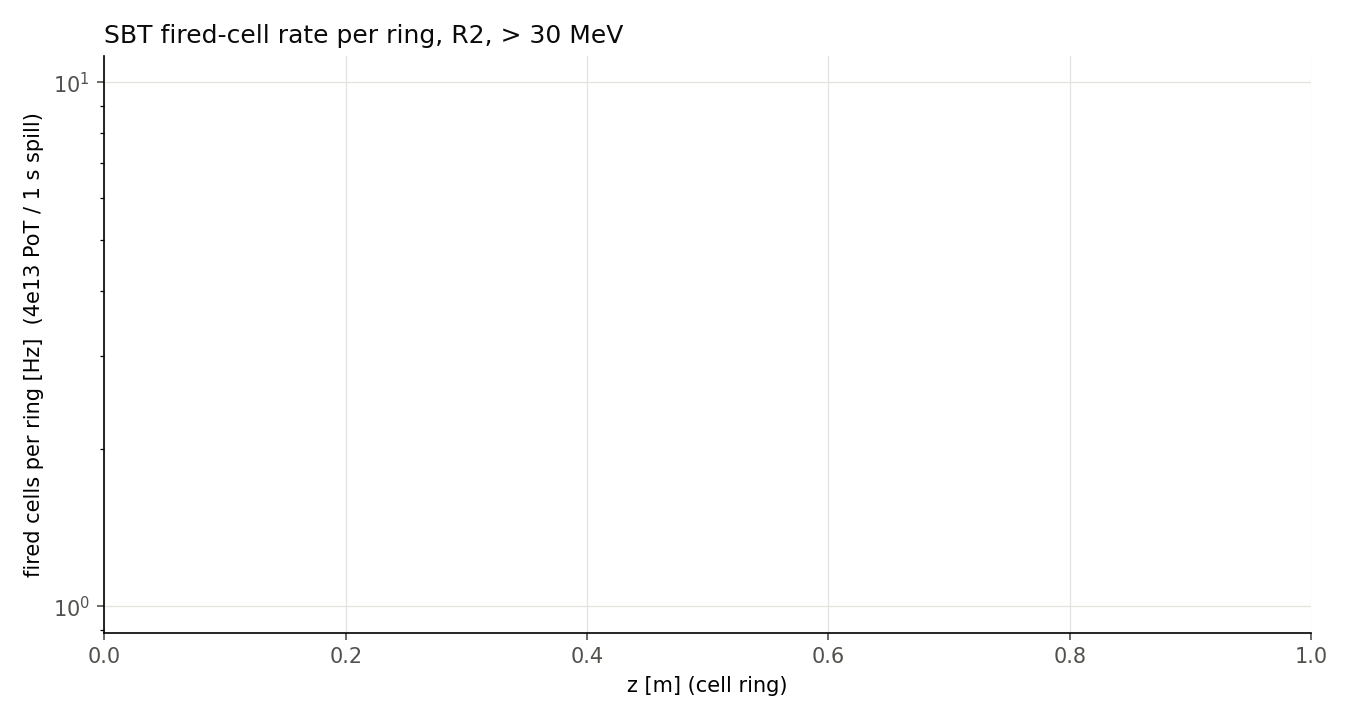
\includegraphics[width=0.80\linewidth]{figs/s41_sbt_firing_rate_per_ring.png}\par}
\vspace{2.46pt}
{\fontsize{6.15pt}{8.60pt}\selectfont
\begin{itemize}
  \item Muons crossing the shell: 2.07 MHz of fired cells (×4 in R2 for back-scatter and e / γ)
  \item ν DIS products: \tbd{} Hz; μ DIS products: \tbd{} Hz
\end{itemize}}
\slidenote{All events, 4×10\textsuperscript{13} PoT per 1 s spill; per cell ring (all four faces). Source: veto results\_rerun/sbt\_firing/summary.md.}
\end{btframe}

% ---------------------------------------------------------------- slide 41c: wall maps
\begin{btframe}{7 · Back-up · SBT firing maps}{Where on the walls: fired cells per class (faces unrolled)}
{\centering 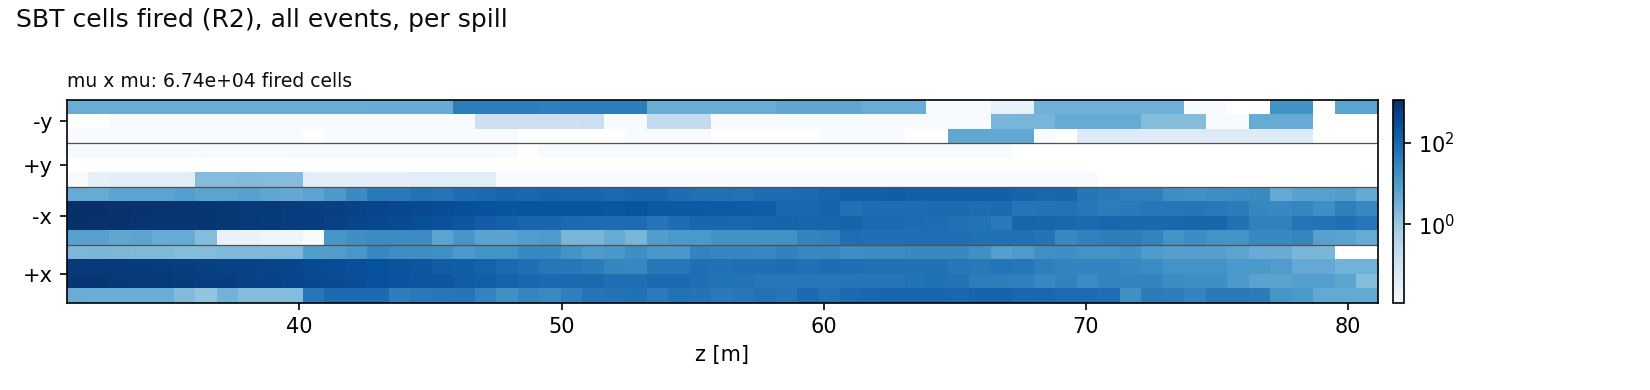
\includegraphics[width=0.86\linewidth]{figs/s41_sbt_firing_wall_map_all.png}\par}
\slidenote{Rows: +x and −x faces (4 cells across), +y and −y (3 cells); columns: the 61 cell rings. Muons and DIS: all events, per spill; μ × μ: the SST1 muons. Source: veto results\_rerun/sbt\_firing/figures.}
\end{btframe}

% ---------------------------------------------------------------- slide 41d: response of the selected candidates
\begin{btframe}{7 · Back-up · SBT firing, selected}{Selected candidates: how often their own particles fire the SBT}
{\fontsize{4.92pt}{6.40pt}\selectfont\setlength{\tabcolsep}{3.06pt}\renewcommand{\arraystretch}{1.42}
\begin{tabularx}{\linewidth}{>{\raggedright\arraybackslash}Xlrrlr}
\textcolor{muted}{class} & \textcolor{muted}{IP cut} & \textcolor{muted}{/ 15 y} & \textcolor{muted}{≥ 1 cell fired} & \textcolor{muted}{fired by} & \textcolor{muted}{mean cells} \\\headrule
ν DIS & < 2.5 m & \tbd & \tbd & \tbd & \tbd \\\rowrule
ν DIS & < 10 cm & \tbd & \tbd & \tbd & \tbd \\\rowrule
μ DIS & < 2.5 m & \tbd & \tbd & \tbd & \tbd \\\rowrule
μ DIS & < 10 cm & \tbd & \tbd & \tbd & \tbd \\\rowrule
μ × μ & < 2.5 m & 31.6 & 97.7 \% & μ\textsuperscript{+} 86 \%, μ\textsuperscript{−} 82 \%, both 71 \% & 7.5 \\\rowrule
\rowcolor{tint}μ × μ & < 10 cm & 1.68 & 98.0 \% & μ\textsuperscript{+} 91 \%, μ\textsuperscript{−} 26 \%, both 19 \% & 5.1 \\\rowrule
\end{tabularx}\par}
\vspace{3pt}
{\fontsize{6.15pt}{8.60pt}\selectfont
\begin{itemize}
  \item μ × μ: every fired cell is upstream of the vertex (the muons come from upstream), where the pointing rule looks; muon deposits sit at the 123 MeV cap of a grazing track (one ring length)
  \item μ × μ at IP < 10 cm: the μ\textsuperscript{+} leg fires the SBT 3.5 × more often than the μ\textsuperscript{−} leg (field polarity of the shield; to be checked)
\end{itemize}}
\slidenote{Before tagging. μ × μ weight = w\textsubscript{a} w\textsubscript{b} × 2 Δt / T\textsubscript{spill} × spills in 15 y (Δt = ±200 ps); 95 k / 14 k MC pairs. Source: veto results\_rerun/sbt\_firing/summary.md.}
\end{btframe}

% ---------------------------------------------------------------- slide 41e: shapes
\begin{btframe}{7 · Back-up · SBT firing shapes}{How many cells, where with respect to the vertex, how much energy}
{\centering 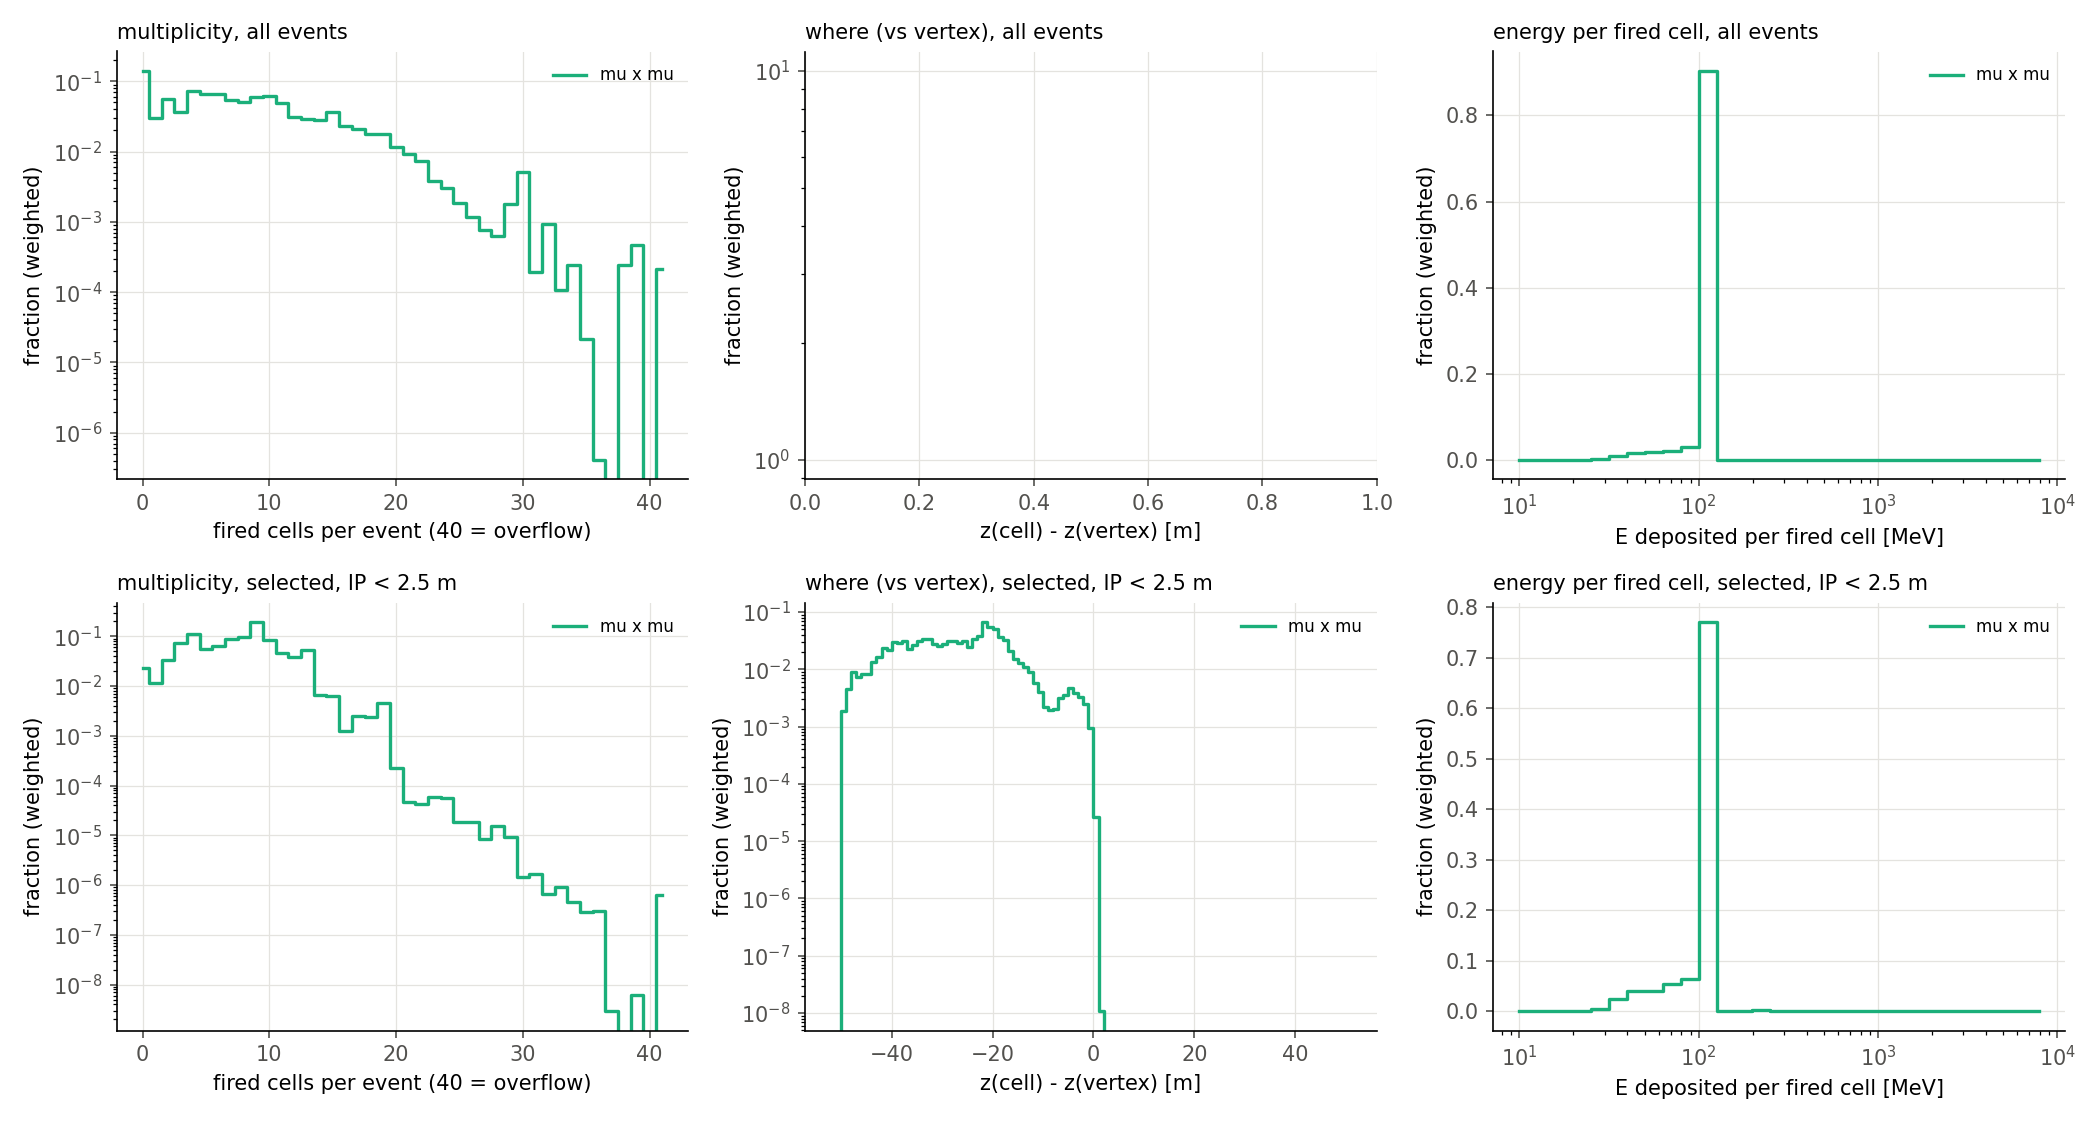
\includegraphics[width=0.90\linewidth]{figs/s41_sbt_firing_shapes.png}\par}
\slidenote{Top: all events; bottom: selected, IP < 2.5 m. Normalised, weighted. Source: veto results\_rerun/sbt\_firing/figures/shapes.png.}
\end{btframe}
